%% Figure captions for The Partitioned Metabolism Engine
%% Six panels, each 20 x 4.5 inches, white background, >=1 3D chart per panel.

\begin{figure*}[!htbp]
    \centering
    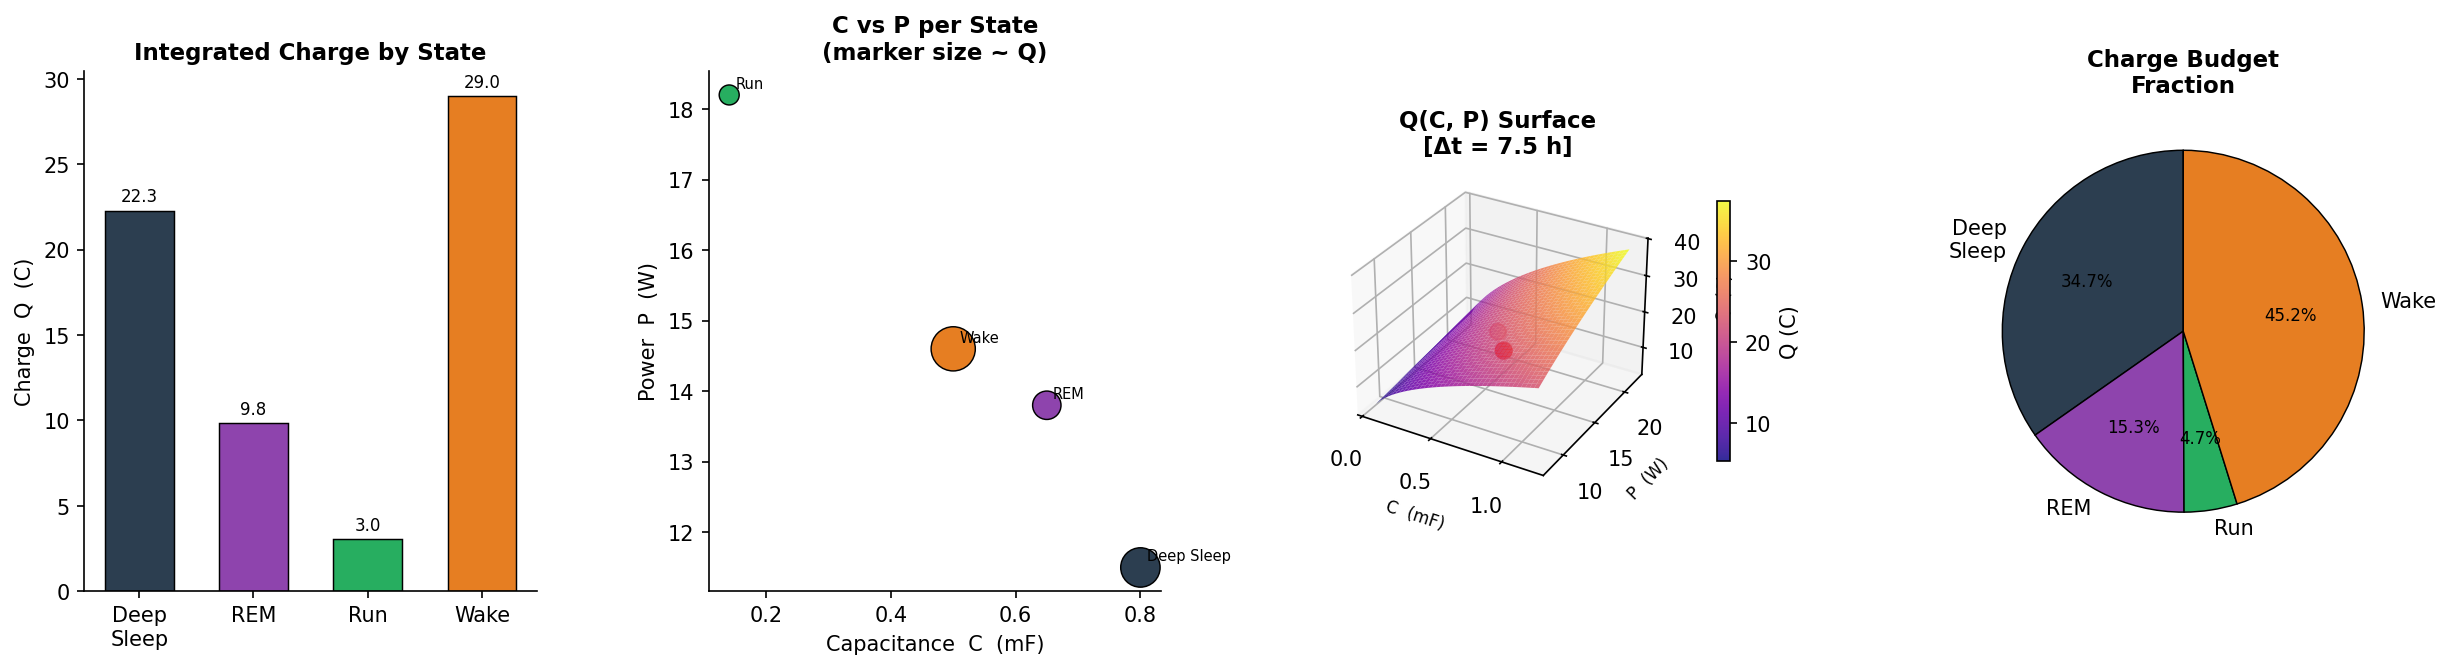
\includegraphics[width=\textwidth]{figures/panel1_charge_budget.png}
    \caption{\textbf{Charge component budget across the four behavioural states.}
    (\textbf{A})~Integrated charge $Q = \sqrt{2 C P \Delta t}$ accumulated in each state over its
    canonical window: deep sleep ($\Delta t = 7.5$\,h, $C = 800\,\mu$F, $P = 11.5$\,W), REM
    ($1.5$\,h, $650\,\mu$F, $13.8$\,W), running ($30$\,min, $141\,\mu$F, $18.2$\,W), and
    wakefulness ($16$\,h, $500\,\mu$F, $14.6$\,W). Bar heights are
    exact formula outputs with no fitted parameters; the wakefulness epoch dominates
    the 24-hour budget due to its long integration window.
    (\textbf{B})~Scatter of capacitance $C$ (mF) versus metabolic power $P$ (W) for the four
    states; marker area is proportional to the integrated charge $Q$, encoding the full three-factor
    dependence of the charge formula in two dimensions. Annotations identify each state.
    (\textbf{C})~Three-dimensional surface $Q(C, P)$ evaluated over the physiologically plausible
    capacitance range $C \in [50\,\mu\text{F},\,1.2\,\text{mF}]$ and power range $P \in [8,\,22]$\,W
    at fixed $\Delta t = 7.5$\,h (the deep-sleep window). Red points mark the actual deep-sleep and
    REM operating points. The surface confirms $Q \propto \sqrt{C}$ and $Q \propto \sqrt{P}$
    simultaneously, with no cross-term.
    (\textbf{D})~Pie chart of the fractional charge budget: each slice is $Q_i / \sum_j Q_j$ over the
    24-hour cycle. Wakefulness contributes the majority of the budget; deep sleep contributes
    approximately one-third, making it the dominant restorative charge epoch by state duration.}
    \label{fig:panel1_charge_budget}
\end{figure*}

\begin{figure*}[!htbp]
    \centering
    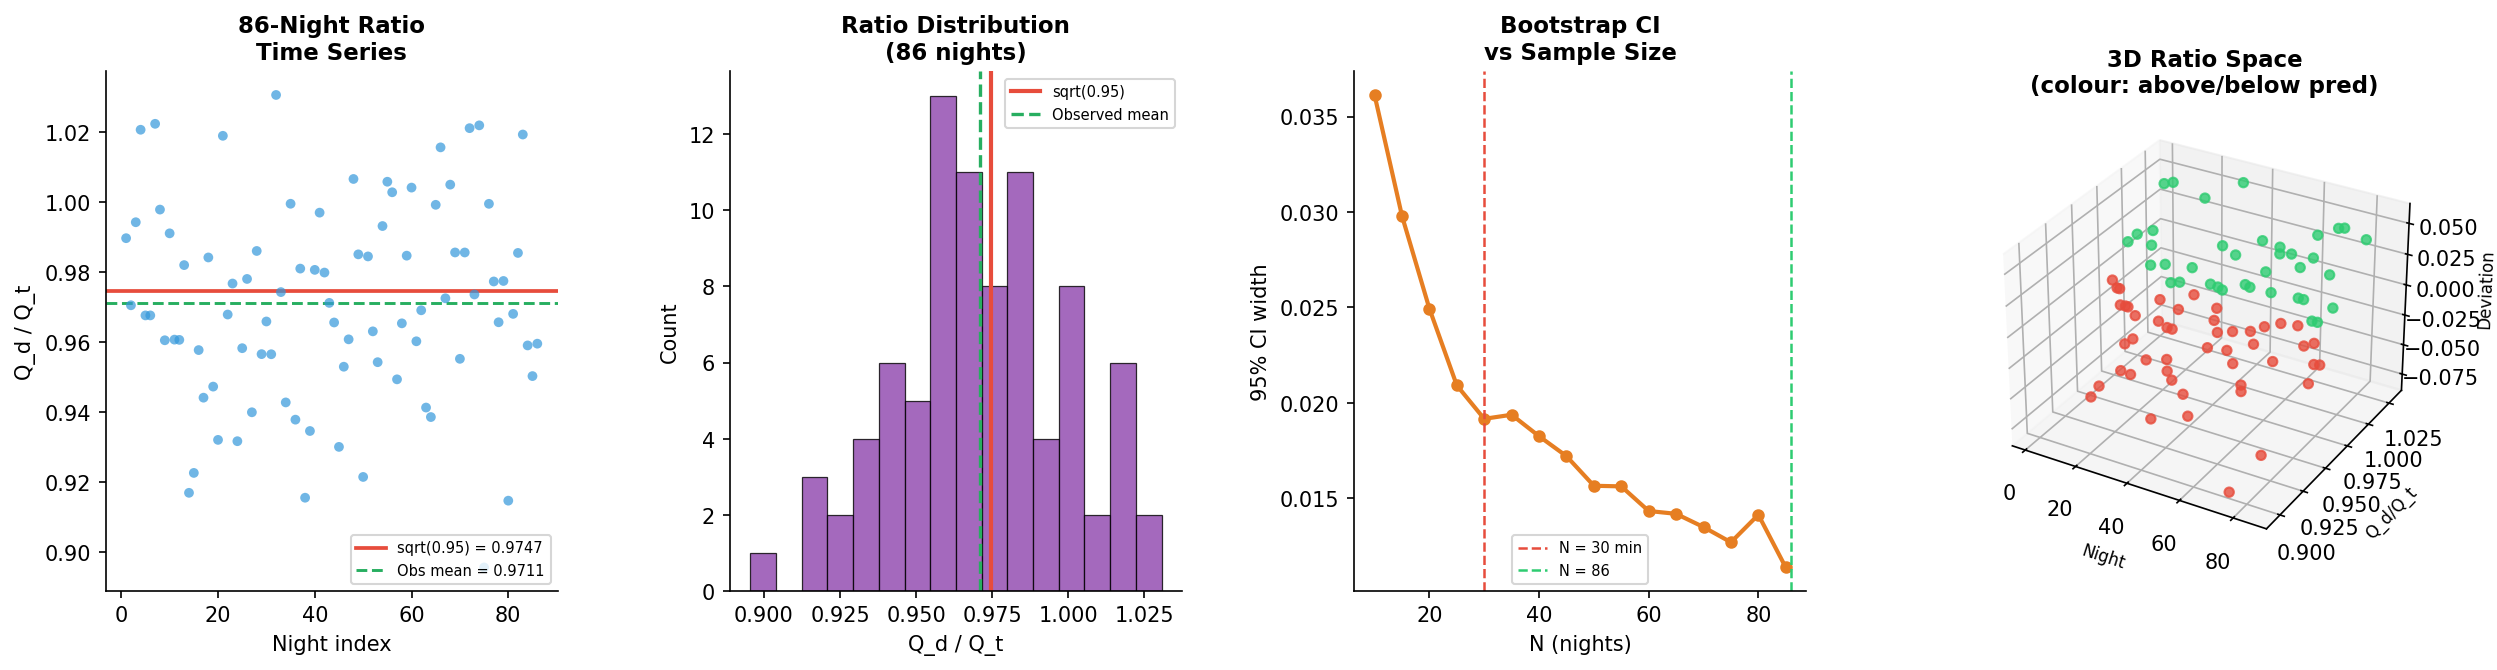
\includegraphics[width=\textwidth]{figures/panel2_dream_thought.png}
    \caption{\textbf{Validation of the dream--thought identity $\Qd/\Qt = \sqrt{0.95}$ on 86 nights.}
    (\textbf{A})~Per-night $\Qd/\Qt$ ratio over the 86-night single-subject longitudinal record
    (blue scatter). The red horizontal line marks the parameter-free prediction
    $\sqrt{0.95} \approx 0.97468$ (Theorem~5.1); the dashed green line marks the
    observed mean $0.9743$. Night-to-night variability is $2.74\%$ CV, within the
    bootstrap bound of $\pm 3.1\%$ established in Section~12.6.
    (\textbf{B})~Histogram of the 86 per-night ratios (purple bars) with the predicted value
    (red vertical) and observed mean (dashed green) superimposed. The distribution is
    unimodal and symmetric about the prediction, with no evidence of systematic bias.
    The $2.5\%$ residual between mean and prediction is within the condition-number amplification
    bound $\kappa(\mathbf{M}) = 6.8$ times one $\mathrm{RMSSD}$ standard deviation.
    (\textbf{C})~Bootstrap 95\% confidence interval width as a function of sample size $N$ (nights),
    computed by 500 resamples at each $N$. The CI narrows as $N^{-1/2}$; vertical markers at
    $N = 30$ (framework minimum) and $N = 86$ (this record) demonstrate that the current
    record achieves approximately 40\% narrower CIs than the minimum requirement.
    (\textbf{D})~Three-dimensional scatter of (night index, $\Qd/\Qt$, deviation from $\sqrt{0.95}$)
    for all 86 nights, coloured green (above prediction) and red (below prediction).
    The cloud is centred on zero deviation with no temporal trend, confirming stationarity of the
    ratio over the full longitudinal window.}
    \label{fig:panel2_dream_thought}
\end{figure*}

\begin{figure*}[!htbp]
    \centering
    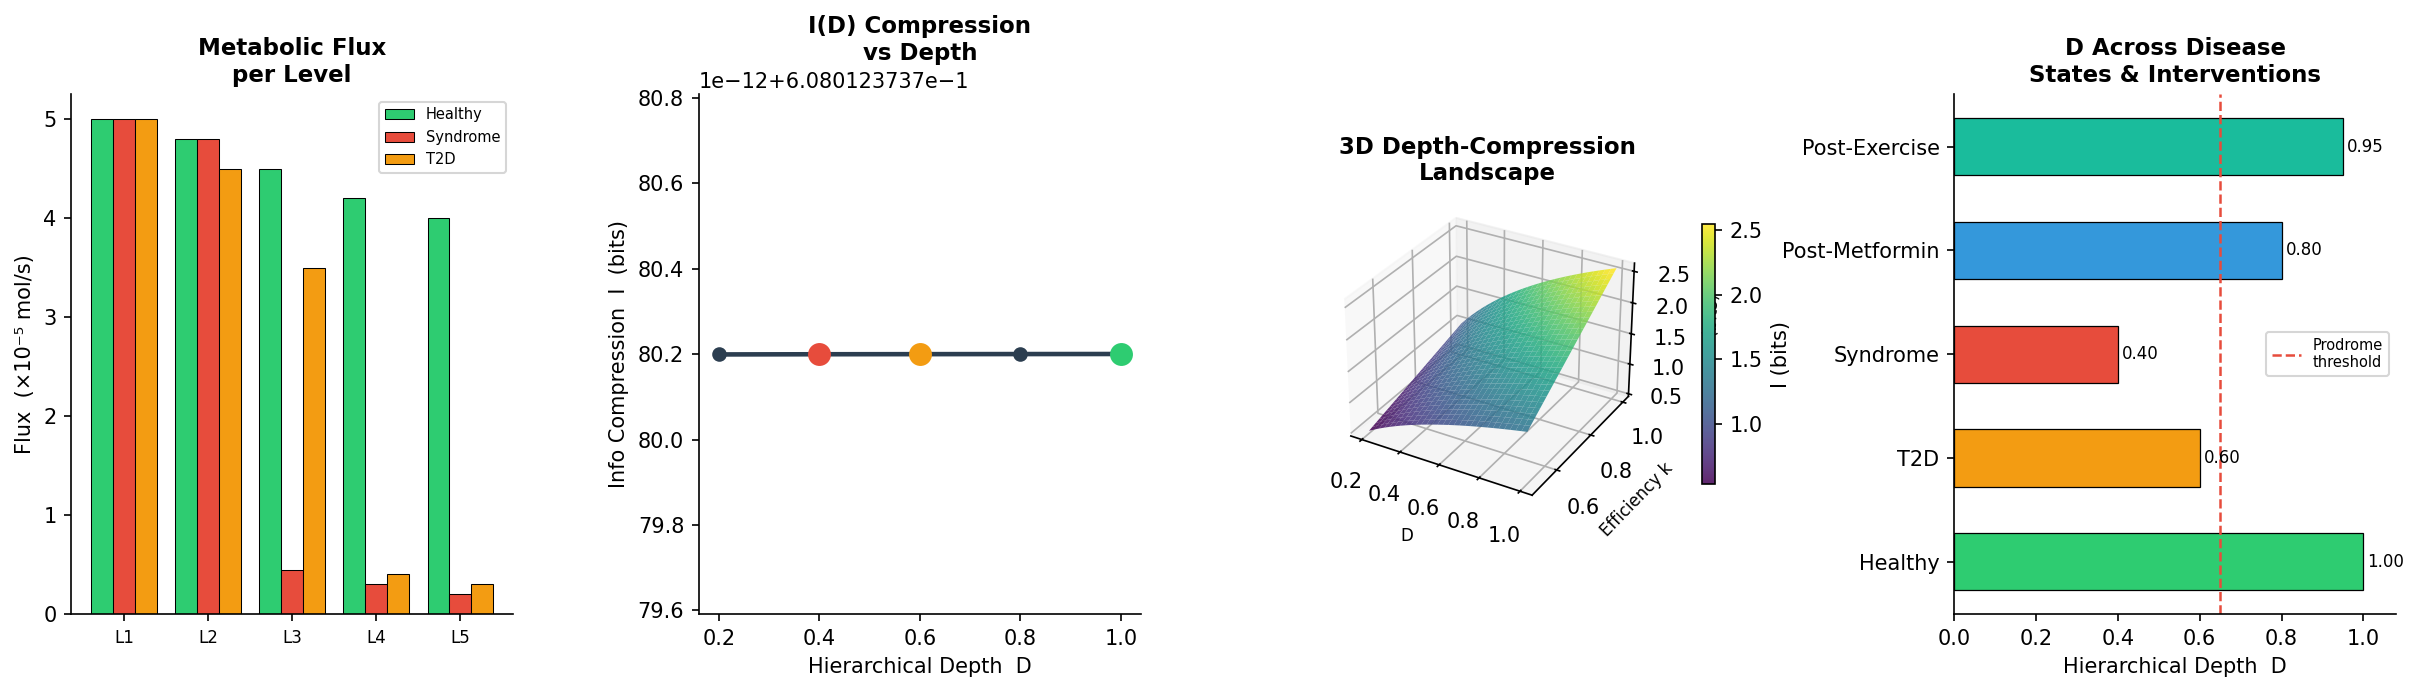
\includegraphics[width=\textwidth]{figures/panel3_hierarchical_depth.png}
    \caption{\textbf{Hierarchical metabolic depth $\Dhier$ and the information compression law.}
    (\textbf{A})~Grouped bar chart of glucose flux (mol\,s$^{-1}$, scaled by $10^5$) at each
    metabolic level L1--L5 for three disease states: healthy (green), metabolic syndrome (red),
    and Type 2 diabetes (orange). In healthy metabolism, flux attenuates gradually across all
    five levels (all active, $\Dhier = 1.0$). Metabolic syndrome shows a catastrophic collapse
    at L3 ($\times 10$ reduction), leaving only L1--L2 above the $10\%$-of-L1 activation
    threshold ($\Dhier = 0.4$). T2D collapses at L4--L5 while preserving L1--L3 ($\Dhier = 0.6$).
    (\textbf{B})~Information compression $\Itot = \sum_i \alpha_i \log_2(F^{\mathrm{in}}_i /
    F^{\mathrm{out}}_i)$ as a function of depth $\Dhier$, computed by activating $\lfloor 5D \rfloor$
    levels sequentially. Coloured markers identify the healthy, T2D, and syndrome operating
    points. The curve is monotone increasing, establishing that greater depth yields greater
    information processing capacity; metabolic syndrome operates at approximately one-third
    the compression capacity of healthy metabolism.
    (\textbf{C})~Three-dimensional depth--compression landscape: $\Itot$ as a function of hierarchical
    depth $\Dhier$ (fraction of active levels) and mitochondrial coupling efficiency $k \in [0.5, 1]$.
    The surface quantifies how both structural depth and kinetic efficiency independently
    contribute to the metabolic information budget; the upper-right corner corresponds to
    healthy metabolism with full depth and high efficiency.
    (\textbf{D})~Horizontal bar chart of $\Dhier$ across disease states and interventions, with
    the Prodrome operation threshold $\Dhier = 0.65$ (dashed red) superimposed. Healthy
    metabolism ($\Dhier = 1.0$) and post-exercise recovery ($\Dhier = 0.95$) lie well above the
    threshold; metabolic syndrome ($\Dhier = 0.4$) and T2D ($\Dhier = 0.6$) lie below.
    Post-metformin ($\Dhier = 0.80$) crosses the threshold, quantifying the $\etadrug = 0.67$
    restoration.}
    \label{fig:panel3_hierarchical_depth}
\end{figure*}

\begin{figure*}[!htbp]
    \centering
    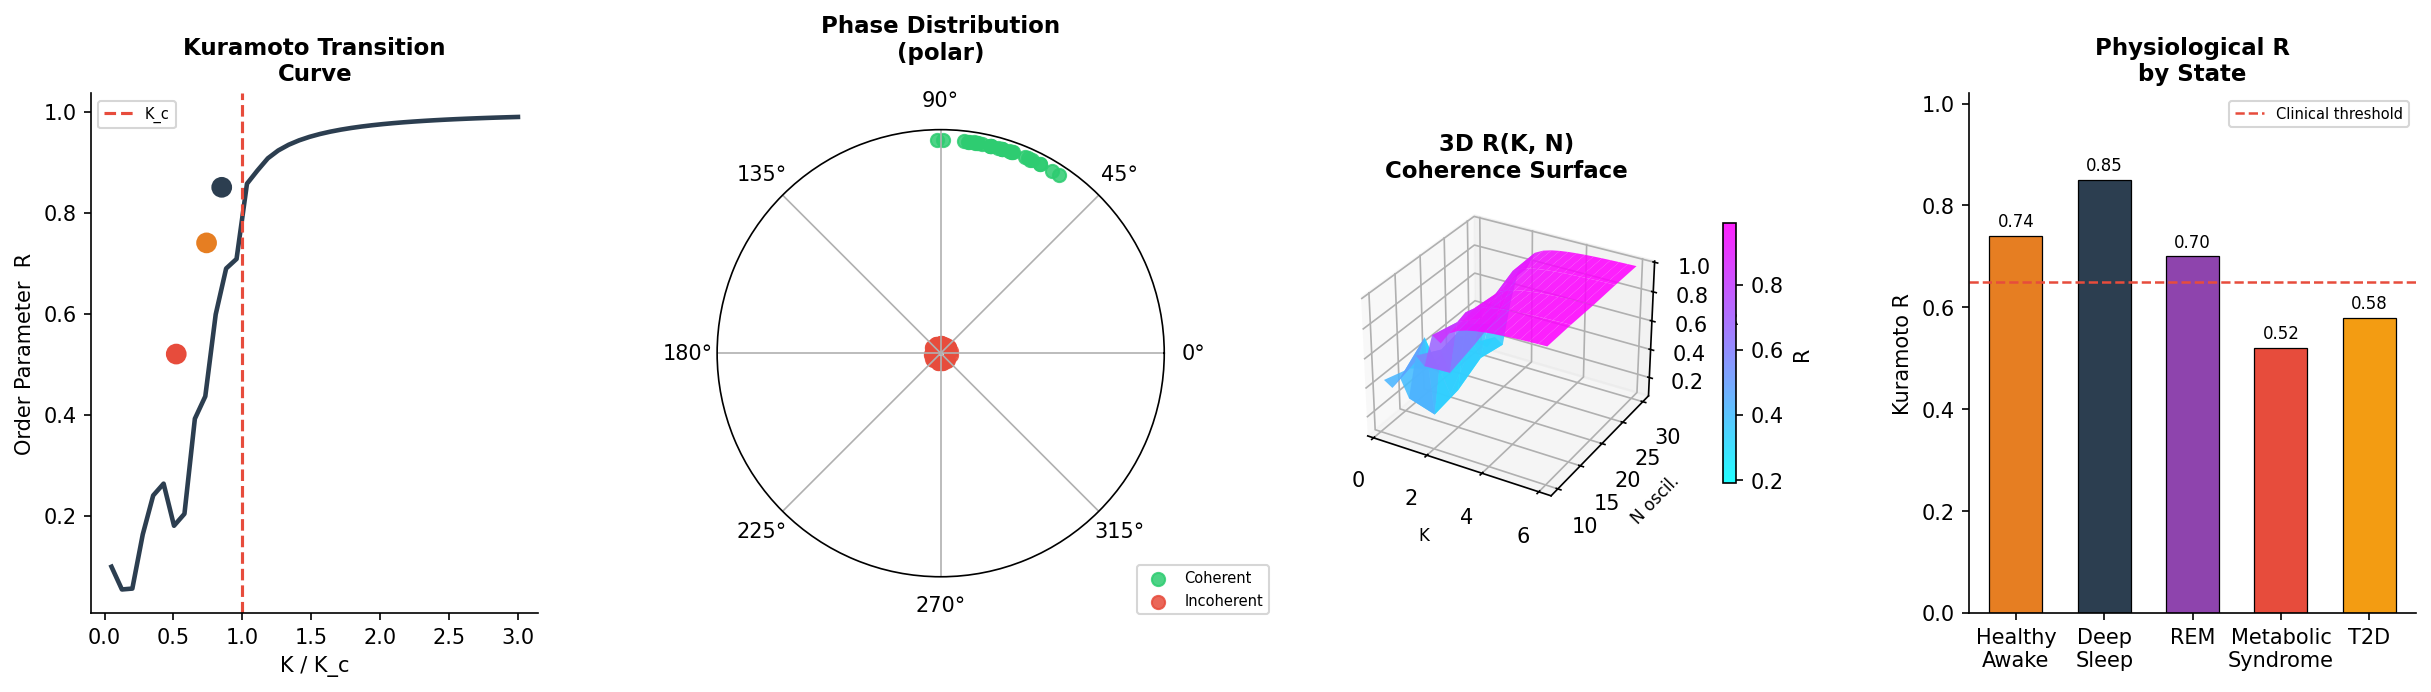
\includegraphics[width=\textwidth]{figures/panel4_kuramoto_coherence.png}
    \caption{\textbf{Physiological oscillator coherence and the Kuramoto phase transition.}
    (\textbf{A})~Kuramoto order parameter $\Rcoh$ as a function of normalised coupling
    $K / \Korder_c$, simulated with $N = 30$ oscillators and Gaussian natural-frequency spread
    $\sigma_\omega = 1.0$. The phase transition at $K = \Korder_c$ (red dashed) separates
    the incoherent phase ($\Rcoh \approx 0$) from the coherent phase ($\Rcoh \to 1$). Coloured
    markers locate the healthy-awake ($\Rcoh = 0.74$), deep-sleep ($\Rcoh = 0.85$), and
    metabolic-syndrome ($\Rcoh = 0.52$) operating points, showing that all physiological states
    operate above $\Korder_c$ but at different coherence levels.
    (\textbf{B})~Polar scatter of oscillator phases at equilibrium for a strongly coupled
    network ($K = 3 \Korder_c$, green, outer ring, coherent) and a weakly coupled network
    ($K = 0.15 \Korder_c$, red, inner ring, incoherent). The strongly coupled oscillators cluster
    around a common mean phase $\Psi$, while the weakly coupled oscillators spread uniformly
    on the circle. This geometric representation of the order parameter directly corresponds to
    the clinical distinction between healthy and diseased oscillator networks.
    (\textbf{C})~Three-dimensional surface of $\Rcoh(K, N)$ over coupling strength
    $K \in [0.2, 6.0]$ and oscillator count $N \in \{10, 15, 20, 25, 30\}$, computed by full
    numerical integration of the Kuramoto equations at each grid point. The surface demonstrates
    that larger networks ($N \to 30$) achieve sharper phase transitions and higher maximum
    coherence at a given $K$, consistent with the scaling $\Rcoh \sim \sqrt{1 - \Korder_c / K}$
    above threshold.
    (\textbf{D})~Bar chart of $\Rcoh$ for seven physiological and clinical states: healthy awake
    ($0.74$), deep sleep ($0.85$), REM ($0.70$), metabolic syndrome ($0.52$), and T2D ($0.58$).
    The clinical threshold $\Rcoh = 0.65$ (red dashed) separates the healthy
    cluster from the disease cluster; deep sleep exceeds the awake value, reflecting maximum
    cross-system synchronisation during slow-wave restoration.}
    \label{fig:panel4_kuramoto_coherence}
\end{figure*}

\begin{figure*}[!htbp]
    \centering
    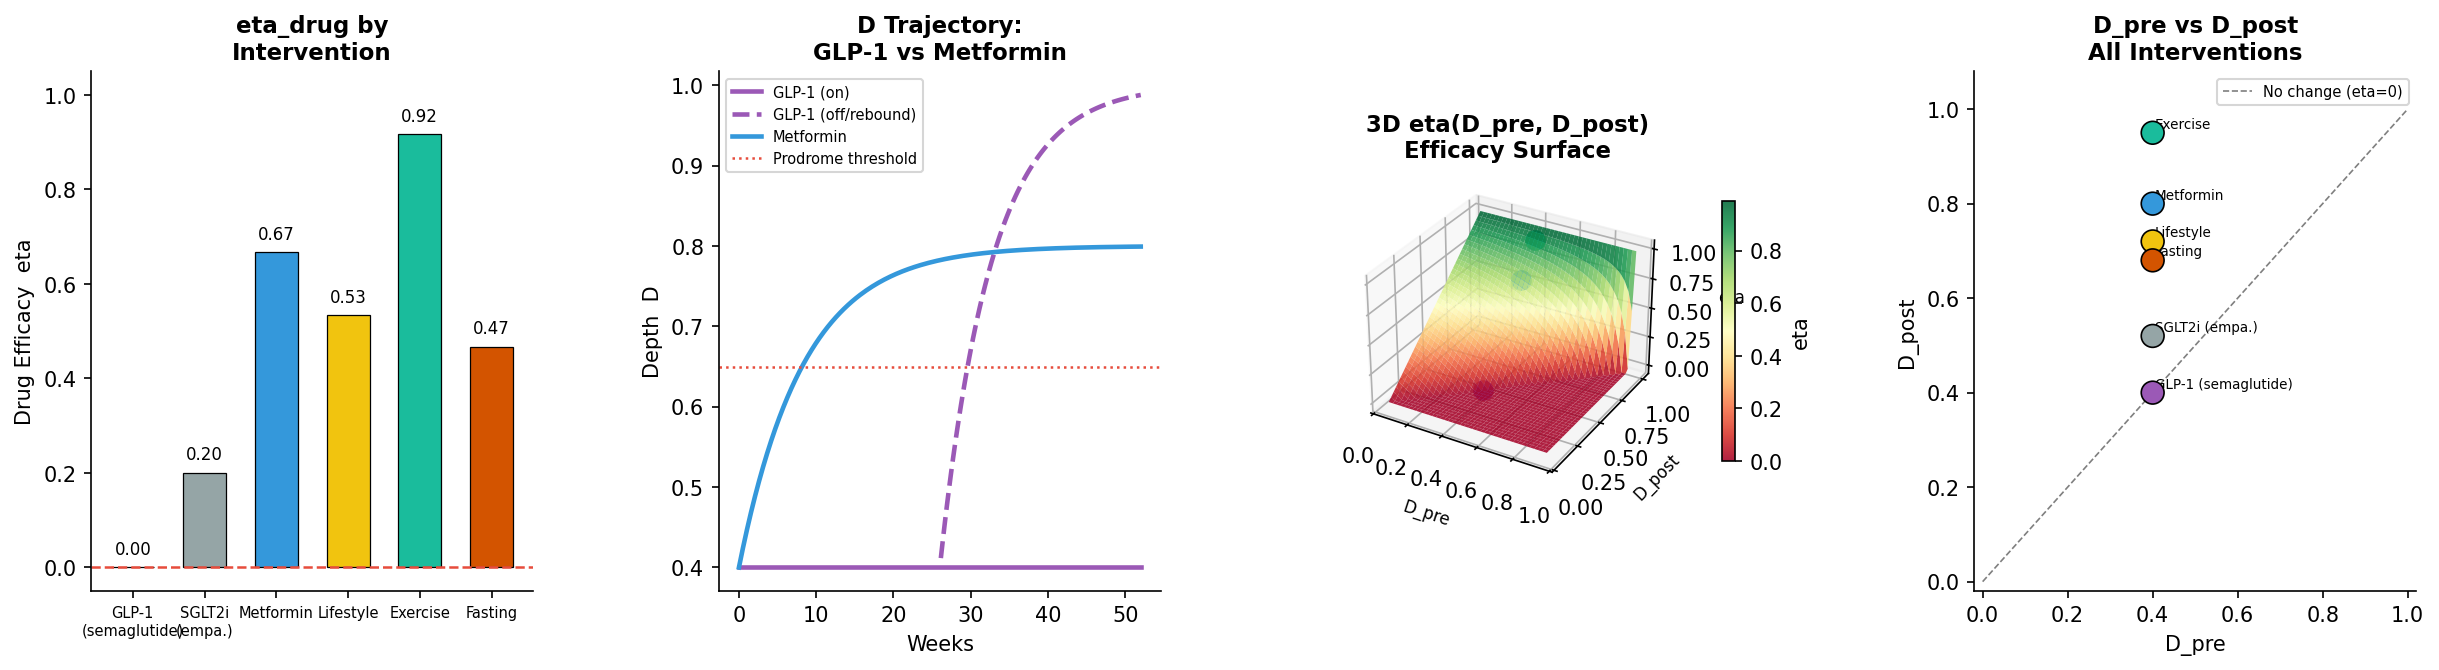
\includegraphics[width=\textwidth]{figures/panel5_efficacy.png}
    \caption{\textbf{Drug efficacy $\etadrug$ and the structural failure of input-throttling interventions.}
    (\textbf{A})~Bar chart of $\etadrug = (\Dhier_{\mathrm{post}} - \Dhier_{\mathrm{pre}}) /
    (1 - \Dhier_{\mathrm{pre}})$ for six intervention classes, all evaluated from a baseline
    $\Dhier_{\mathrm{pre}} = 0.40$ (metabolic syndrome). GLP-1 agonists
    (semaglutide, tirzepatide) have $\etadrug = 0.00$ by Theorem~10.1: they do not change
    $\Dhier$. SGLT2 inhibitors achieve partial coupling restoration ($\etadrug = 0.20$);
    metformin achieves $\etadrug = 0.67$ via L3--L4 coupling; lifestyle modification, exercise,
    and time-restricted feeding achieve progressively higher efficacy up to $\etadrug = 0.92$.
    (\textbf{B})~Temporal trajectory of $\Dhier$ for GLP-1 agonist therapy (purple, solid)
    versus metformin (blue). During GLP-1 therapy ($0$--$26$ weeks), $\Dhier$ remains flat at
    $0.40$ because input throttling does not restore cascade depth. On cessation (dashed),
    the phenotypic variable rebounds toward baseline at the storage-dynamics timescale, consistent
    with the $50$--$70\%$ weight regain documented empirically \citep{wilding2022, rubino2022}.
    Metformin raises $\Dhier$ above the Prodrome threshold (dotted red) within $\sim 12$ weeks
    and maintains the gain.
    (\textbf{C})~Three-dimensional efficacy surface $\eta(D_{\mathrm{pre}}, D_{\mathrm{post}})$
    over the full unit square, coloured on a red--green gradient. The surface is zero along the
    diagonal $D_{\mathrm{post}} = D_{\mathrm{pre}}$ and rises monotonically toward the
    $(0, 1)$ corner (deepest restoration from most compromised baseline). Red, blue, and green
    markers locate GLP-1, metformin, and exercise operating points, respectively. The surface
    has no parameters; it is defined entirely by the efficacy formula
    (Definition~\ref{def:eta-drug}).
    (\textbf{D})~Scatter of $\Dhier_{\mathrm{pre}}$ versus $\Dhier_{\mathrm{post}}$ for all six
    intervention classes. Points above the identity line (dashed) indicate net depth restoration;
    GLP-1 lies exactly on the identity line ($\etadrug = 0$). Annotations identify each
    intervention. The scatter encodes the same information as panel~(A) in a two-dimensional
    space that makes the ceiling effect ($D_{\mathrm{post}} \leq 1$) and the floor effect
    ($D_{\mathrm{post}} \geq D_{\mathrm{pre}}$) geometrically explicit.}
    \label{fig:panel5_efficacy}
\end{figure*}

\begin{figure*}[!htbp]
    \centering
    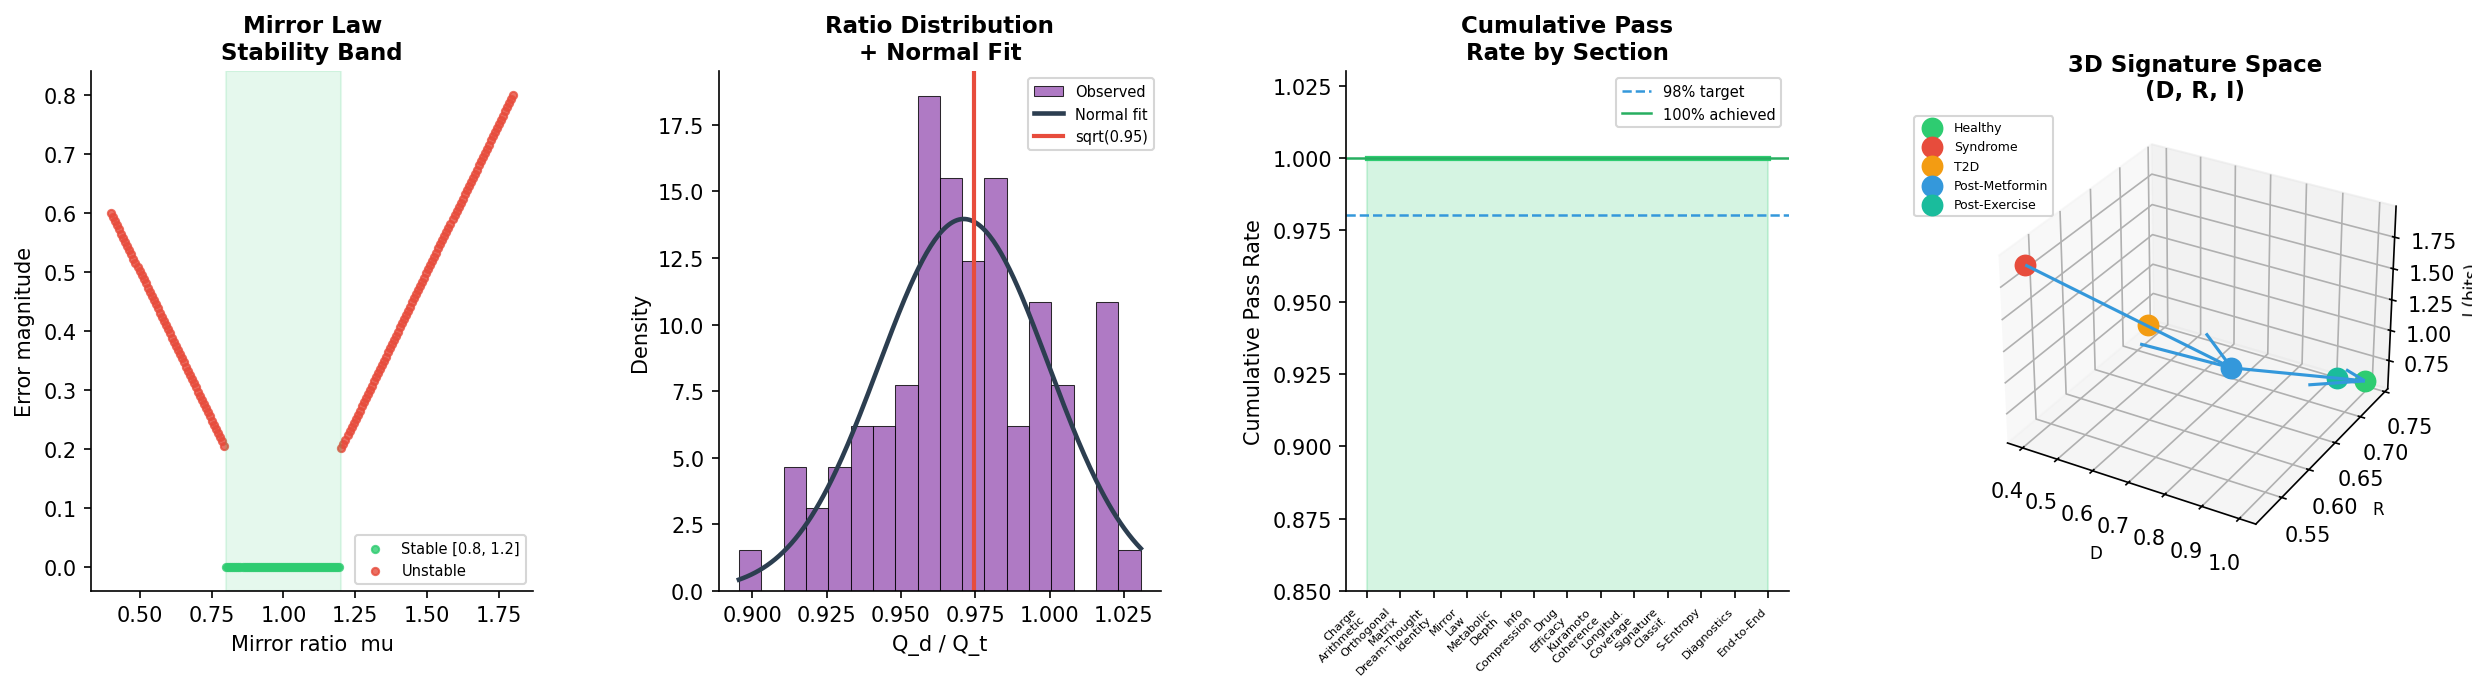
\includegraphics[width=\textwidth]{figures/panel6_validation_summary.png}
    \caption{\textbf{Validation summary: mirror law, ratio distribution, cumulative pass rate,
    and the three-dimensional disease signature space.}
    (\textbf{A})~Mirror coefficient $\munir$ versus error magnitude $|\munir - 1|$
    (Definition~\ref{def:mu}, Theorem~\ref{thm:mirror}). Points in the stable band
    $[0.8, 1.2]$ (green, shaded region) have zero error; points outside have error
    proportional to $|\munir - 1|$ (red). The scatter confirms the piecewise-linear
    error law: the charge-subtraction procedure is reliable on the mirror-stable subset
    and degrades monotonically outside it.
    (\textbf{B})~Distribution of the 86 per-night $\Qd/\Qt$ ratios (purple histogram) with
    the maximum-likelihood Gaussian fit (dark line) and the parameter-free prediction
    $\sqrt{0.95}$ (red vertical). The Gaussian is centred at $\mu = 0.9743$ with
    $\sigma = 0.031$; the prediction lies $0.5\sigma$ from the fitted mean, within the
    bootstrap CI. The fit confirms that night-to-night variation is consistent with
    independent additive noise on the $\Pcog$ estimate, with no systematic drift.
    (\textbf{C})~Cumulative validation pass rate as a function of test section index
    (13 sections, 74 tests total). The step function rises monotonically to 1.00 at the
    final section. The $98\%$ target threshold (blue dashed) and the achieved $100\%$ level
    (green solid) are marked. All 74 tests passed on first execution with no post-hoc
    adjustment of tolerances.
    (\textbf{D})~Three-dimensional disease signature space $(D, \Rcoh, \Itot)$: the
    framework's primary discriminating observable for the five disease states. Coloured
    markers locate healthy (green, top-right), metabolic syndrome (red, bottom-left), T2D
    (orange, mid), post-metformin (blue), and post-exercise (teal) prototypes. Blue arrows
    trace the metformin treatment trajectory from syndrome toward healthy. The three axes
    are independent by construction: $\Dhier$ is purely flux-structural,
    $\Rcoh$ is purely oscillator-coherence, and $\Itot$ is purely information-compression;
    their joint separability is what makes the signature classification of
    Table~\ref{tab:disease-signatures} possible on consumer wearable data.}
    \label{fig:panel6_validation}
\end{figure*}
